
\chapter{Embedded ML Infrastructure for Plasma Characterization}
\label{section:4_embedded_ML}

It has been shown in the introductory chapter the diversification of signals within their heterogeneous nature, however a particular discussion should be also addressed to the possible domain of the data itself beyond the particular origin.
In order to provide high quality descriptions of the plasma properties during a the pulse in a fusion experiment session a wide amount of sensors are usually required, both in time and in spatial domains.
Although it is not true that controllability (and observability) of the system strictly depends on that amount of inputs; the overall description of a complex system, indeed, is usually led by few driving signals~\cite{Liu2011}. 
This definition agrees with the intuitive notion of control that, for a properly structured system, the appropriate manipulation of few variables are a sufficient information to drive the whole behavior; like in the bike riding example where the actual only two control variable are the steering of the handlebar and the torque on the pedals. 

Even if the complete environment of all the variables that must be observed to provide a optimal control on the system states is rather complex, it can be shown\cite{Lesort_2018}~\cite{an2019unsupervised} that a properly configured latent variables can effectively generate a simpler embedded representation. This in turn led us to start evaluating the possibility to a simpler control model that would take inputs from the latent states instead of directly depending on the whole detectors.
Such a system would be possible only if many sub-systems of the experiment diagnostics would apply these ML techniques and cooperate to a unified embedded representation. This is rather a long shot scenario that is currently difficult to foresee in a concrete implementation, however some small steps could have been done exploiting the already ongoing changes of RFX-mod2.

A new setup of the magnetic probes is under study for the experiment, combining the structural upgrade of the conductive shell with the redesign of the magnetic sensor system, to gain a more detailed access at the Magneto Hydro Dynamic (MHD) processes that take place into the plasma~\cite{zuin2009current}~\cite{innocente2014tearing}.
Part of the study that has been carried out during this research regarded the possible adoption of a fully digital solution, using a configurable FPGA to handle ADC conversion and providing a set of on-line functions including the realtime numeric integration and signals recording.

This fits well with the possibility of eventually apply also more sophisticated algorithms that are not handled by the central CODAS only but also in the peripheral devices that compose the acquisition front-end. 
However the fundamental prerequisite is to achieve a compact and reliable implementation of such algorithms, and in particular for the encoder-decoder networks that attain the latent embedding. This must embrace a clever selection on both the hardware and software component of the acquisition system. In this chapter a proposal for a new DAQ chain is presented, together with the early results for the new magnetic acquisition system in RFX-mod2. Then, in~\cref{section:quantum}, a method to embed the neural network in such devices is explained.


\subsection{New "smart" devices in DAQ chain}
\label{section:daq-chain}

In the context of a concurrent interest on data analysis and control in plasma experiments, a good implementation for an acquisition device should provide a double result: on one side it should act as a transparent recorder on the raw data that comes from the sensor, on the other side it should prepare a compact useful signal that can be used for the control.
The first requirement is evidently motivated by an off-line investigation on the recorded physical quantity, where characteristic of the signal could be eventually modified a posteriori from external information ( a custom analysis algorithm, or a better definition of the sensor/signal characteristics ). 
The real-time control on the other hand has completely different requirements, being the timing constraints the key factor to provide a proper feed-back action. It needs to provide a concrete elaborated output right in a given time.

In addition a pre-processing of the signal in the embedded design should provide a way to tune its characteristics. This does not hold in general for a transient recording device, where we are interested in maintaining a coherency on the signal history, but it is a key factor for controlling experiment, where we needs to modify parameters in the seek for new operative states. This is also particularly true in the perspective of applying neural networks because the training on new acquired data and/or change the layers structure bust be accounted.

A good candidate FPGA technology was recently proposed and gained lot of interest as a possible solution for integrating both flexibility and performance. It comes from the market of embedded systems and exploit the \ac{SoC} fabrication technique to host a standard processing unit with an FPGA logic in the same silicon device.
An example is the \textit{Xilinx Zynq} system, integrating a \textit{Kintex-7} family FPGA together with \textit{ARM-A9} CPU cores. 
We based our study on this kind of chips being one of the most widespread adopted soultions, and because it is relatively cheap.

The duality of the processing system (PS) and the logic unit (PL) in the same chip presents many advantages. Many common subsystems, such as memory controller and IO ports, are handled by dedicated hardware. The ARM processor is also able to run a full featured operative system (like GNU Linux) at full performance, handling a possible high-level communication with other devices, with the storage system, or for central experiment control. 

\begin{figure}
    \centering
    \includegraphics[height=6cm]{img/4_EmbeddedML/zynq_schema.png}
    \caption{A schematic diagram of all Zynq-7000 All programmable SoC components, with the available interconnection ports for PS/PL communication.}
    \label{fig:zinq-7000}
\end{figure}

It allows to set-up a self-contained acquisition board with a drastic simplification of the system, providing both the autonomous local storage for high throughput transient recording functions, as well as the ability to send real-time decimated and integrated data to the control servers through standard gigabit Ethernet interface. 

Among the possible realtime pre-processing that can be developed, the flexibility provided by a configurable on board FPGA allows also the inclusion of more sophisticated triggering mechanisms, and a deeper integration with the timing systems. Examples of triggering mechanism are given by the acquisition of fast transients requiring high speed sampling only in a given, dynamic Region of Interest (ROI). This feature has been implemented in the first proof-of-concept device described in a later section and already used in the NIO1 experiment\footnote{The NIO1 experiment is a compact and modular negative ion source built at Consorzio
RFX, with the aim to investigate the optimal configuration for a negative ion source for \acs{NBI} systems} as reported in Appendix~\cref{section:NIO1}. Deeper integration with the timing systems imply the ability of getting the clock and the trigger signals not only from digital inputs, but also from the specifically coded signal carrying both clock and trigger information (timing highway)\cite{dio4}. Such signals were used in the RFX-mod timing systems to distribute a synchronous clock and asynchronous triggers and a timing device was required for every ADC rack to extract the clock and the trigger signals. The timing device is no more required for a rack hosting the new ADC devices because the ADC devices can directly extract timing information from the timing highway. This will at the same time reduce the board population on cubicles and make the possible stand-alone operation of such devices for small experiments or placing electronics in critical sites.
%
The cited Zynq architecture has been provided in this research by the Red Pitaya board~\cite{redpitaya}, currently used for the development and tests. A different solution is however foreseen for the production system where an external ADC section with the Zynq-based module will be integrated in a custom carrier board. 
An ADC front end, already used in other applications of real-time plasma control~\cite{ATCA-MIMO-ISOL}, has been considered and it is presented in the next section. 
The first implementation of the flexible ADC architecture has been carried out on a Red Pitaya board, using the in-board ADC channels, and it is already operating for small applications (see appendix). Even if not intended to represent the final application, development of FPGA logic on Red Pitaya offers the advantage of a ready-to-use ADC channel in a compact and inexpensive solution. Most of the firmware design will be retained in the final implementation, using a different ADC front end. 

The real opportunity behind the use of FPGA technology for real-time is twofold: it provides a concrete possibility to fully parallelize tasks without need of any synchronization or preemption because the resulting component are completely independent logic; and for each implemented process the execution time is absolutely deterministic, depending only on the signal propagation through ports. Moreover the actual definition of the latency of each function can be precisely estimated ahead of time during the logic syntesis. 

In a hybrid processor and logic units solution like the Zynq SoC for the design of a multipurpose ADC device the tasks can be divided in two categories, addressing the time critical operations to the logic, and the "less critical" function to the high level software components running in the CPU.
Examples of time critical functions that are carried out by the FPGA in this context are:
\begin{itemize}
\item The management of a circular data buffer and the DMA transfer in RAM of pre-trigger and post-trigger samples in transient recording;
\item anti-aliasing filtering and subsequent sub-sampling of the samples to be streamed in real-time. The resulting samples are enqueued in a FIFO accessed by the processor;
\item any digital filtering and preconditioning of the signal, for instance the required digital integration for deriving magnetic field measurements from EM probe signals;
\item ROI detection in case ADC triggers are derived from the signal itself (e.g. over a given signal level threshold);
\item Clock and trigger extraction in case a highway signal is provided by the timing system, encoding both clock an triggers.
\end{itemize}
%
The less critical functions addressed to the processor unit are:
\begin{itemize}
\item The management of the configuration setting, received via TCP/IP. The processor validates the configuration and write the related registers in the FPGA;
\item off-line data readout of acquired samples in transient recording and communication via TCP/IP with the central data acquisition system;
\item network data streaming of sub-sampled data read from the FIFO and sent in UDP packets to the active plasma control system. 
\end{itemize}

This subdivision is also schematically represented in \Figure{\ref{fig:daq}} where an example of this digital acquisition is inserted in a representation of the magnetic acquisition chain and closed control loop from sensors to actuators. 
The schema reports on the left an array of input channels represented by the sensor coils connected to the analog to digital frontend. The digital signal is digitized and subsequently serialized in a high speed \ac{LVDS} line that is connected to FPGA. The serialization is needed to reduce the number on ports occupation on the FPGA input, but specially to also add a line galvanic insulation that, being on the digital side, does not affect the frequency response of the port.
All serialized inputs are subsequently entering in the FPGA logic, where a interface circuit is responsible to handle the serial communication and to convert the stream of data in a AXI4 Stream protocol\footnote{AXI stands for } \cite{AXI4}. Internally the AXI bus connects the interface to a custom logic that is the site of the internal elaboration, and the target of a possible ML implementation. This component is the able to access to io ports or to talk to the system via \ac{DMA} access to memory or register FIFO buffers.
%
Data buffering, DMA engine, I/O FIFO and registers are generally held by standard codes provided by Xilinx and tailored on the specific hardware access we are using. In the custom component three VHDL sub-blocks carry out the underlying logic. The first block provides the management of clock and triggers that may be either directly derived from digital inputs or rebuild by properly decoding the timing highway input signal. The second block provides programmable input signal elaboration such as low pass filtering for subsampling and integration. The third block will handle the triggering logic and the circular buffer holding pre and post trigger samples. In particular, the trigger may be derived from external signals (via the first block) or derived from the input signal (e.g. when the input level is greater than a given threshold).    

\begin{figure}[ht]
\centering
%\includegraphics[width=0.9\textwidth]{img/4_EmbeddedML/schema_logico.pdf}
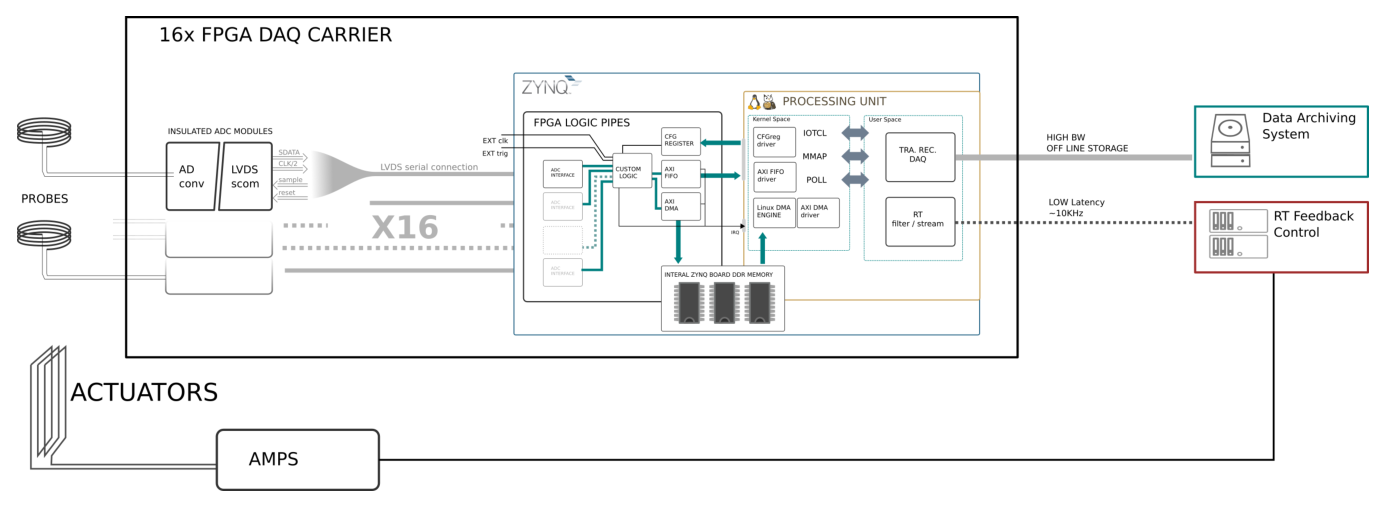
\includegraphics[width=0.9\textwidth]{img/4_EmbeddedML/DAQ_chain.eps}
\caption{Logic design of the flexible ADC structure.}
\label{fig:daq}
\end{figure}

Communication of subsamples streamed data for real-time plasma control is achieved using the XILINX AXI Stream FIFO. The Xilinx "\textit{AXI Stream FIFO}" is a Xilinx free software IP that implements a read/write FIFO queue with a well defined communication protocol. A proper connected IRQ line is used to trigger events to the processing unit together with the related set of status and enable registers. In this way data samples are readily available to the linux processor and will be sent using low latency UDP communication to computing nodes carrying out distributed for real-time plasma control. 
Conversely the communication of the data acquired at high speed in the ROI is carried out by a DMA engine, using circular DMA buffers in order to minimize the number of data copies. In this case data will be sent to the central Data Acquisition system via TCP/IP as soon as a ROI has been acquired.





\section{ EM signal acquisition }

The electromagnetic instant characterization of the machine represents the base and the reference for almost any diagnostic in a fusion experiment and in particular at RFX. 
The current pick-up coils acquisition chain comes from a long machine operation experience, where all the electrical characteristics of components have been tailored on the acquired signals. In particular the system is composed by two separate sets of ADC channels, one for precision transient data sampling, dedicated on off-line analysis of plasma perturbations, and one for real-time control. The observed physical quantity is the local magnetic field vector that is reconstructed by orthogonal coils providing both $B_r(t)$ and $B_t(t)$. These are the main observed quantities related to the MHD perturbation, the third component can be easily computed using $\Vec{\nabla} \cdot \Vec{B} = 0$.
%
\begin{figure}
    \centering
    \subfigure[]{\includegraphics[width=0.49\textwidth]{img/rfx/conditioning_circuit.png} \label{fig:pomaro_integrator}}
    \caption{The RFX-mod signal conditioning and analog integrator for magnetic pick-up coils acquisition. }
    \label{fig:my_label}
\end{figure}
%
The field is obtained on each channel by direct analog integration~\cite{pomaro2005transducers}, the schema of such analog system is reported in~\Figure{\ref{fig:pomaro_integrator}}. As shown it can be conceptually divided three main groups: the magnetic sensor itself, the signal conditioning front-end, and the final analog integrator.
The front-end acts as a differential amplifier that removes the common mode noise on the signal ( it can very severe in the RFX experiment due to the large magnetizing flux variation ) and adds a filter to remove aliasing and to compensate the signal transmission line response.
The analog integrator solution was selected at that time because of the fast variation of the signal with respect to the available sampling frequency. 

Among the RFX-mod2 experiment upgrades~\cite{Peruzzo2018} a substantial improvement of the magnetic measurement system is foreseen. The total number of the new magnetic pick-up coil sensors will be much higher with the aim of an improved spatial resolution~\cite{marchiori2017upgraded}. 
The sensors will be also moved inside the vacuum vessel widening their usable signal bandwidth up to 200~kHz. These characteristics are meant to provide a better view on the fast reconnection events that generate the QSH status. Beside the structural challenges that came with a such redefinition of the vacuum vessel, and the increased complexity of the sensors system setup and cabling, these changes imply demanding requirements for the acquisition system also. 

The direct extension of the present analog integration would result non trivial and expensive. The changed requirements in bandwidth indeed ask for a redesign of the integrator, and the increased number of channels that would require a readjustment of the available cubicle space.
Thus a more compact and cost effective solution is being investigated. 

Given the recent advances in digital acquisition systems that are facing the market the posibility to switch the current design to a digital integrator seems to be feasible. A valuable ready to use solution could be based on the ATCA-MIMO-ISOL~\cite{carvalho2010reconfigurable} architecture originally developed for the plasma column vertical stabilization of the JET tokamak experiment and already tested on RFX-mod~\cite{manduchi2012upgrade}. 
The acquisition channels of this architecture are isolated input modules using precision 18-bit, 2~MSamples/s SAR ADC coupled to an FPGA which then routes the data flow to the processing/storage servers through a PCI-e interface.

These characteristics of high sensitivity and high serial throughput, combined with the galvanic insulation of the input section of each module make it very interesting for the proposed application target.
At such an acquisition rate this architecture could be able to perform the numeric integration needed for the current real-time plasma control configuration, while simultaneously recording the $dB/dt$ signals suitable for the study of the fast MHD dynamic processes taking place into the plasma~\cite{zuin2009current}~\cite{innocente2014tearing}. 
The possibility of directly acquiring the time derivative of the electromagnetic fields, i.e. the direct signals from EM probes, was not present in the previous system. All magnetic channels were composed by already integrated signals in order to reduce the number of required ADCs. However this fact introduces a severe limitation in the derivative control required for MHD stabilization because of the bad quality of the computed time derivative.

However for our purposes, the ATCA/PCI-e architecture is still expensive and complex to manage. Although it has been equipped with an onboard FPGA of the Xilinx Virtex-5 family, almost the entire design is reserved for the sole acquisition and the software and firmware has been tightly fitted to its original scope. A certainly more safe approach is to take advantage of the good design of the acquisition front-end using a more simple and flexible architecture of the FPGA board. 

Therefore the acquisition chain has been set based on the ADC design described in the previous section using the Zynq system. This approach promises also a further reduction of the number of ADC channels because it will be able to perform high frequency transient recording in local memory (up to 1 MHz), and lower frequency streaming (up to 10 kHz) required for real-time plasma control, having a single ADC channel for both.




\subsection*{EM channel characterization}

To assess the feasibility of this proposal, we developed an interface adapter between the MIMO ISOL ADC module and the new acqusition device mounting a Zynq-7000 SoC, and then we investigated the limits of the direct numeric integration technique with presently available electronic components.
The goal is to check to what extent a directly acquired signal from the RFX-mod2 probes can be digitally integrated. Even if applied to this specific case, the results obtained here could be used as guidelines for other similar applications as well. 

\begin{figure}
    \centering
    \includegraphics[width=0.49\textwidth]{img/4_EmbeddedML/ATCA_MIMO_ISOL_schema.png}
    \caption{Schematic of the digital frontend of the ATCA-MIMO-ISOL acquisition system at JET.}
    \label{fig:portoghese_schema}
\end{figure}

The required dynamic range specifics ask for a careful evaluation of both the minimum detectable and the maximum expected signal, keeping in mind that the signal has to be integrated numerically.  
The maximum level of the signal can be straightforwardly derived from experimental measurements that have been already carried out on RFX-mod operation, which can be used to estimate the level of the signal once the probe characteristics and its measurement chain are defined. 
The probes used up to now on RFX-mod~\cite{pomaro}~\cite{pomaro2005transducers} present a typical sensing area of 0,025 m2 and proved to offer a good compromise between compactness, signal sensitivity and usable bandwidth. The new probes of RFX-mod 2 will maintain these basic geometric and electric features, while the materials and the manufacturing process will be modified to comply with the new vacuum installation~\cite{MARCHIORI2017892}. 
An example of the expected $dB/dt$ signal source plotted in time and frequency, obtained by wide-band in-vessel probes installed on RFX-mod, is shown in Fig.\ref{fig:em_signal_raw}.
%
\begin{figure}[ht]
\centering
\subfigure[]{\includegraphics[width=0.45\textwidth]{img/4_EmbeddedML/1.png} \label{fig:em_signal_raw_a}}
\subfigure[]{\includegraphics[width=0.45\textwidth]{img/4_EmbeddedML/2.png} \label{fig:em_signal_raw_b}}
\caption{example of dB/dt signal of the toroidal field component from an in-vessel wide bandwidth probe from a reversed field pinch pulse at 1.5 MA in RFXmod-2 (a), the frequency spectrum realted to the same signal (b).}
\label{fig:em_signal_raw}
\end{figure}
%
The same data source signal has been used to set the maximum signal level of the dynamic range requirement.
The final desired range is actually high because, on the other hand, the minimum signal level is an important feature as well: it involves the sensitivity to slowly changing magnetic field at low intensity. 
Magnetized plasmas are prone to amplify the spatial resonant components of external fields. So even small unwanted field variations (the so called “field errors”) can have large effects on the whole plasma behavior and must be actively corrected (e.g. by \textit{compass scan} error field correction).
In addition this ability to detect small field components is also needed to allow the detection (and correction) of the misalignment between the sensors and the structure. 

One of the unavoidable and yet challenging issue of the electromagnetic field measurement is the $1/f$ background, or \textbf{pink noise} associated to any electronic device.
It is a signal with a frequency spectrum such that the power spectral density (signal energy per frequency interval) is inversely proportional to the frequency.
The principal sources of pink noise in ADC devices are associated to the slow fluctuations of the condensed-matter properties in the device components. These include fluctuating metal defects configurations, changing of the occupancies in semiconductors, and the domain structures in magnetic materials. The explanation for the $1/f$ shape turns to be related with the distribution of kinetic activation energies of the fluctuating processes.
The electronic pink noise is unavoidable, and there is no known lower bound to this background in electronics. Measurements made down to $10^{-6}$ Hz (with several weeks of acquisition) have not shown a ceasing of pink-noise behaviour.

This reflects to the integration results as a low frequency envelope \textbf{drift} that can affect the measure of small field components even in few seconds.
As a reference the performance of noise level and integrator drift of the actual conditioning system of RFX-mod is shown in Fig.~\ref{fig:rfx-mod_drift_b}. The final integration error is of the order of 0.6 mT, with the typical signal range to be measured which spans from 10 mT to 0.5 T. Some of the integration drift error can be corrected in post-processing, but it is necessary to keep it into an acceptable range to allow the use of these signals for real-time control purposes.
%
\begin{figure}
\centering
\subfigure[]{\includegraphics[width=0.4\textwidth]{img/4_EmbeddedML/3.png} \label{fig:rfx-mod_drift_a}}
\subfigure[]{\includegraphics[width=0.4\textwidth]{img/4_EmbeddedML/4.png} \label{fig:rfx-mod_drift_b}}
\caption{RFX-mod analog integrators after 10 sec. Two integrated signals examples (a), and the distribution of final integration errors from toroidal field sensors on 8 “dry” pulses (1510 signals) (b).}
\label{fig:rfx-mod_drift}
\end{figure}


The analog to digital conversion inside each of the ATCA-MIMO-ISOL board ADC modules is delegated to an Analog Devices AD7641, a 18-bit SAR converter that acquires signals from a fully differential input in the range $\pm 10$V at the maximum rate of 2~MSamples/s. A block scheme of the module is shown in Fig.~\ref{fig:portoghese_schema}. The initial preconditioning of the signal is quite similar with the current RFX-mod version, the analog input is filtered by a 1 pole, 100 kHz passive component connected to a differential amplifier THS4520 used as input range adapter.
The signal is the fed into a high precision ADC: the Analog Devices AD7641 that provides a serialized output to the galvanic insulator.
At the end the digital stream is opportunely converted to LVDS to be properly sent to the FPGA ports. Both the power supply and the digital output are insulated: the former with a DC/DC converter, which is synchronized with the ADC conversion start command in order to minimize the noise spikes generated during power switching phase, the latter with an high speed GMR component\footnote{A galvanic insulator that exploits the Giant Magneto Resistence effect, ref.\cite{Hirota2002}}.

The module has been subsequently interfaced with the Zynq FPGA board, developing a custom HDL code with the purpose of streaming data output to a proper embedded GNU Linux driver. Fig. \ref{fig:em_channel_hdl} shows the schematic design of the bus connections of the FPGA logic.
\begin{figure}[ht]
\centering
\includegraphics[width=0.7\textwidth]{img/4_EmbeddedML/7.png}
\caption{block scheme of the implemented Zynq Xilinx AXI driver}
\label{fig:em_channel_hdl}
\end{figure}
Each picured box, commonly refferred as IP block (Intellectual Property block), represents an HDL code ( usually it can be written either in Verilog or VHDL ) where the links are the connection among the input registers and output ports of all the involved components.
Two main IP symbolic components are visible: the first one from the left of the sketch represents the processor entity, the second is related to the module digital acquisition. The processor unit presents two bus connections, externally linked to the DRR and fixed I/O hardware components, and one internally connected by the AXI\_GP0 general purpose bus to the other custom logics. Here all the IRQ and clock connections have been hidden to improve the schema readability but all the components are clocked by 125MHz Zynq internal multiplier and the FIFO drives an interrupt of the PS to inform the driver of the status changes. The custom logic named scc52460\_fifo encloses all the implemented design exploiting a 32-bit Xilinx AXI-Stream FIFO core with the input connected to a chain of custom cores performing in sequential order: the acquisition from module LVDS serial port, a configurable decimation of acquired data, and a configurable length packetization of the output stream. The communication protocol selected in the schematic hardware design of ADC module is the AD7641 serial master WARP mode connection with a further external flip-flop connected to the clock output that makes the signal transaction dual edge synchronized (rising and falling). This aims at achieving, likewise the DDR protocol specification, the same throughput with half of the frequency that in this way matches the one of the signal data.  The read implementation approach is then a double buffers with two process that have the sensibility to the respectively rising and falling edge of the SCLK\_in clock input port. On the other side a proper kernel module has been developed implementing the Xilinx FIFO core communication protocol~\cite{axi4_stream_fifo_2016}, in this way the kernel spools data from the FIFO buffer to the user allocated memory. Other solutions could be certainly applied to read data from the device, for example the Zynq is equipped with two high speed embedded DMA channels that are able to write data directly into DDR relieving the CPU of the mem-copy load. The proper transfer architecture should be always chosen in relation with the overall project complexity and goals. The system has been then tested for long lasting acquisition pulses at full speed 2 MSPS output and it resulted to be able to work properly in continuous mode. 

Once built the interface to the FPGA we could gather signals directly in the system internal storage, here operated as a MDSplus device.
Being the final target the input signal integration, we carried out a detailed characterization of the noise seen by the ADC. Each run consisted of 8 noise snapshots, each one lasting 40 s ($8\cdot107$ samples). In order to reduce extraneous components, known noise sources have been either switched-off or kept far from the ADC board. The modules used have been configured to have an input signal range of 10.3 V.
The noise has been characterized in time \Figure{\ref{fig:dcdc_noise_a}} and histogram of the reconstructed value code (i.e. the direct word read from ADC, not yet rescaled to actual physical unit that it represents) in \Figure{\ref{fig:dcdc_noise_b}}. 
In the code distribution two side bands are present and degrade the quality of the measure, this turned out to be caused by a noise component generated by the DC/DC converter. This is visible in the time domain as a series of synchronous spikes, which reflect in the three peaks shown in frequency and the overall larger sigma.
%
\begin{figure}[ht]
\centering
\subfigure[]{\includegraphics[width=0.4\textwidth]{img/4_EmbeddedML/9.png} \label{fig:dcdc_noise_a}}
\subfigure[]{\includegraphics[width=0.4\textwidth]{img/4_EmbeddedML/10.png}\label{fig:dcdc_noise_b}}
\caption{Noise sampling (a), and noise histogram on 100,000 samples (b), of the module in standard configuration with 50 Ohm terminated input. Note the repetitive synchronous spikes and the resulting multi-modal distribution due to the DC/DC converter residual noise.}
\label{fig:dcdc_noise}
\end{figure}

At the same time the module has been inspected in the frequency domain. The result is reported in \Figure{\ref{fig:noise_spectra_a}}.
Two spectra have been plotted: the red showing the noise of the module with "as is", wile the blue plot report the noise acquired with all the preconditioning filter and amplifier bypassed from the circuit.
In the red spectrum two peaks are visible (i.e. the spikes on the right of the figure, one at 500 kHz and its 1 MHz harmonic at Nyquist frequency) and are related to the mentioned isolation DC/DC converter noise. Even if this line on spectrum could be affecting some off-line analysis, those components are not much relevant for the final integration being outside the target bandwidth. On the other hand the real issue is the pink noise level that is quite high for the red plot and reduced for the blue one, thus it seems to come from the analog frontend.
%
\begin{figure}[ht]
\centering
\subfigure[]{\includegraphics[width=0.4\textwidth]{img/4_EmbeddedML/noise_spectra.png} \label{fig:noise_spectra_a}}
\subfigure[]{\includegraphics[width=0.4\textwidth]{img/4_EmbeddedML/17a.png}           \label{fig:noise_drift_b}}
\caption{Noise spectra (spectral levels are power normalized) after disconnecting the input amplifier; left panel circuit fed by its DC/DC converter, right panel by linear power supply – note the suppression of the frequency peak at 500 KHz.}
\label{fig:noise_spectra}
\end{figure}
In \Figure{\ref{fig:noise_drift_b}} a set of integrated EM probe signals has been overimposed in the time domain on a period of 10s. This clearly shows the effect of the 1/f noise in the two cases, showing the concrete drift reduction of the removed electronics.
%
\begin{figure}
    \centering
    \subfigure[]{\includegraphics{img/4_EmbeddedML/18.png} \label{}}
    \subfigure[]{\includegraphics{img/4_EmbeddedML/22.png} \label{}}
    \subfigure[]{\includegraphics{img/4_EmbeddedML/20a.png} \label{}}
    \subfigure[]{\includegraphics{img/4_EmbeddedML/24a.png} \label{}}
    \caption{Noise integrated signals histograms after 10s of ACD acquisition, with and without the input amplifier (a)(b); and two samples of integrated signal compared to a reference without noise in the same situations (c)(d).}
    \label{fig:before_after_correction}
\end{figure}

The study on This module showed the feasibility of a completely digital approach for the electromagnetic probes acquisition in RFX-mod2. We exploited existent hardware from ATCA-MIMO-ISOL system from Jet interfaced to a flexible FPGA SoC Board to learn the communication interface. The noise spectrum revealed that this module is not actually adequate for the purpose of performing the digital integration of the EM signals, thus a further investigation will be required to improve the signal to noise ratio in such architecture. However the chain of acquisition has been successfully built for the system ADC module and FPGA host, proving that the technology is almost ready to provide such digital signal elaboration.
This opened the way to explore other kinds of signal elaborations, such as the introduction of ML algorithms, and will make possible to use all electromagnetic channels to extract plasma state information for the control.

\subsection*{Machine Learning for digital signal conditioning}

In RFX-mod a fixed reduced set of signals from EM probes was used for the active plasma control, requiring a new set of ADC converters in respect to the transient recorders used for data acquisition. In RFX-mod2 it will be possible to re-use any ADC channel from EM probes for real-time control, and the actual number will be only limited by other factors, not related to the ADC devices, such as network bandwidth or control computation load. 

However being the new acquisition based on a flexible FPGA architecture a possible future integration with machine learning algorithm could be speculated.
For example a properly trained autoencoder could perform a compression of the required throughput \cite{Zebang:2019:DCA:3313950.3313965}, making it possible to effectively pass all the needed information though the network to the central control system.
In \cref{section:VAE}, for example, the representation of a complex 40 element features has been reduced to a representative latent variable of only size 2. 
This could be thought as a method for compressing a spatial or time (or both) varying signal into an embedded representation through an encoder network on the sensor front-end, and then this could be re-expanded back to a representation of the original signal on the controller back-end.

In addition, if a complete control based on a neural network will be applied, the embedded representation could be directly used, easing the computational load of the decoder function. This will discussed later talking about the Autoencoder composition.
It is nonetheless worth to mention the fact that, in such a situation, a possible communication of a latent space representation could be also thought to be in the opposite direction. Indeed, if we would succeed to have a complete characterization of the plasma status, a possible backward information could be fed to the sensors to better interpret the read data.
For example in the case of EM probes this could ease the integration drift simply knowing, from all the other sensors, that such a shift of the magnetic field would be unlikely to happen.

This is a very good example of the possible data fusion scenario that neural networks could bring once integrated to the RFX-mod2 acquisition system.
A small step has been initiated from the upgrades that could be applied to RFX-mod2, and the adoption of the discussed "smart" sensors devices.
However this remains a bare intuition unless concrete implementations of a neural networks in FPGA are not demonstrated.
This is the topic of the next section.


\section{Quantized neural networks for embedded implementation}
\label{section:quantum}

In numerical computation we refer to the \textit{quantization} as the process of constraining the number of bit that reproduce a numerical value. In effect any digital number is already intrinsically quantized, in the sense that its representation is defined on a limited discreet domain. Nevertheless, even if the number of bits that are used to represent a digital quantity is finite, and so is the possible set of values that it can assume, the actual position of those values in the target domain is not strictly fixed. This means that we can decide where to place any of possible available reproduction number to fit the desired manifold.

If the function that maps the digital representation with a numerical entity is linear the numerical format can be described by only two parameters: the \textbf{range}, which refers to the range of all possible numbers that can be represented, and the \textbf{precision} that tells how many values can be represented within the dynamic range, which in turn determines the resolution (the distance in the target domain between two adjacent numbers).

In the context of deep learning, and in information theory in general, the predominant numerical format used for both training and final deployment is the floating point, either in 32-bits or 64-bits versions. For a \acs{MLP}, for example, floating point operations involves the linear combination of weights and biases with input features for each layer, and the non-linear activation function. The formulation of floating point numerical format is a very clever solution that adapt the range to the represented number.

Floating-point can be thought in concept similar to the scientific notation. Their numbers consist of a signed set of digits of a fixed length in a given \textbf{base} (the radix), this is referred as the \textbf{mantissa} (or \textit{significand}). The length of mantissa determines the precision to which numbers can be represented. The radix point position is assumed always to be within these given digits in a fixed position, while a signed integer \textbf{exponent} modifies the magnitude of the number.
To finally obtain the actual represented value of the floating-point number the mantissa is multiplied by the base raised to the power of the exponent. This is shifting the radix point from its defined position by a number of places equal to the value of the exponent: to the right if the exponent is positive, or to the left if the exponent is negative.
Symbolically, this represented value can be derived as 
%
$$ (-1)^s \,\, m \times b^e $$
%
where: $s$ is the sign $m$ is the mantissa (absolute value), $p$ is the precision (the mantissa number of digits), $b$ is the base, and $e$ is the exponent.
The standard IEEE-754~\cite{1985--ieee754} is the widely adopted notation for floating points numerical computation, it is defined with base 2 and uses a mantissa with radix point at first digit. In this case both exponent and mantissa are binary numbers, and mantissa has always the first digit equal 1 ( with the sole exception of the representation of the real number 0.0 ). 



% The flexibility introduced by floating point dynamic range is that the numbers can be represented not uniformly spaced; the difference between two consecutive numbers grows with a scale defined by the chosen exponent.





%RR
However given this dynamic mapping of the scale the floating point may require a slight amount of computational resources.
When a processing unit is executing an algorithm where a floating-point operation is not directly supported by the hardware, the CPU tries to use a series of simpler floating-point operations, either by basic internal routines or by means of specific libraries.
In systems without \acs{FP} dedicated hardware, the CPU uses a series of fixed-point arithmetic operations that remain on the processor \ac{ALU}.

For example the currently used convolutional networks in imaging, such as the VGG~\cite{Simonyan15} family, contain over
$1.3\tilde1.4\times10^8$ internal parameters, and require over $15\times10^9$ \acs{FP} operations to classify a single image.

%RR
While CPU and GPU clusters are currently the go-to platforms for CNN and many other machine learning applications, a customized hardware solution on FPGA can offer significant improvements in energy efficiency and power dissipation. These factors may be critical in enabling the increased use of CNNs in low-power settings such as unmanned drones or embedded computing


The steps for performing the floating-point Addition/Subtraction are: 
1) Separate the sign, exponent and mantissa of the inputs, and check whether the inputs are zero, infinity or an invalid representation in the standard. Add the hidden bit to the mantissa.
2) Compare the two inputs: a logical shift right operation must be performed over the smaller of the two numbers. The number of bits of the mantissa shifted right, dependent on the exponent’s difference, and this difference is a preliminary exponent calculation result. Finally, add/sub the current mantissas.
3) Shift left the achieved mantissa until its most significant bit (MSB) is 1. For each shift decreases the current exponent by 1. Finally, concatenate the sign, exponent and mantissa of the final results.

The steps for performing a multiplication are:
1) Separate the sign, exponent and mantissa of the inputs, and check whether the inputs are zero, infinity or an invalid representation in IEEE-754 standard. Add the hidden bit to the mantissas.
2) Multiply mantissas, add exponents, and determine the product sign.
3) Whether the MSB is 1 in the mantissas multiplication result, hence, no normalization is needed. The current mantissa is shifted left until a 1 is achieved. For each shift operation the current exponent is decreased by 1. Finally, concatenate the sign, exponent and mantissa of the final results.


However, if the target is the FPGA implementation, the full IEEE 754 floating point standard~\cite{1985--ieee754} shows to be quite hardware resources demanding in terms of LUT (Look up tables for logic operations), FF (flip flops), and DSP (digital signal processors) counts~\cite{num_lut_for_fp}~\cite{1227254}. 
For example for a 32-bit floating point number the following resources are consumed in a Xilinx Virtex5 family device (xc5vlx110T).
%
\begin{table}[]
    \centering
    \begin{tabular}{l|l|c|c|c|c|c}
        \textbf{Operation} & \textbf{Optimization} & \textbf{LUT-FF} & \textbf{LUT} & \textbf{FF} & \textbf{DSP} & \textbf{Latency} $[ns]$ \\
        \hline
        Add/Sub   & DSP48E  & 354 & 238 & 342 & 2 & 1.0 \\
                  & speed   & 578 & 379 & 602 & 0 & 5.4 \\
                  & latency & 656 & 500 & 668 & 0 & 1.1 \\
                  
        Multiply  &        & 35 & 74  & 5 & 1.7 
    \end{tabular}
    \caption{Caption}
    \label{tab:my_label}
\end{table}

multiply-add \cite{62143}


% RR
The desire for reduced bandwidth and compute requirements of deep learning models has driven research into using lower-precision numerical formats. It has been largely proved that both linear combination and non linear activation can be effectively represented using a fixed point math, in particular 8-bit integers (INT8) have been successfully applied without incurring in significant loss of accuracy. 
But, not enough, the use of even lower bit-widths, such as 4/2/1-bits, is an active field of research that has also shown great results.

















% % CONTROL THEORY
% According to the classical \textit{control theory} for dynamical systems, once the precise time derivative description is given in terms of that state space model, a system can be defined \textit{controllable} if there exist a particular set of inputs that are able to drive the state to any desired \textit{set point} within a finite time. 
% If the classical discreet time \ac{LTI} state space model is considered in the form:
% \begin{align}
%     & \dot{\bm{x}} = A\bm{x} + B\bm{u} + \bm{w}\\
%     & \bm{y} = C\bm{x} + D\bm{u} + \bm{v}
%     \label{eq:ss_model}
% \end{align}
% % \begin{align}
% %     & \bm{x}_t = A\bm{x}_{t-1} + B\bm{u}_t + \bm{w}_t\\
% %     & \bm{y}_t = C\bm{x}_t + D\bm{u}_t + \bm{v}_t
% %     \label{eq:ss_model}
% % \end{align}

% Time dependent state space models in \eqref{eq:ss_model}, also known \acl{DLM}, are a widely used approximation for analyzing time series. They provide a very flexible framework allowing concurrent smooth and steep changes that generally well fitting natural process time evolution.
% A more rigorous formulation for \textit{controllability} is given in terms of the \textit{Kalman criterion}:
% \begin{definition}{Kalman criterion}
% The pair $(A,B)$ is \textit{controllable} if, given a duration $t>0$ and two arbitrary points $x_0, x_t \in \mathbb{R}^n$, there exists a piece wise continuous function $\tau \mapsto u(\tau)$ from $[0,t]$ to $\mathbb{R}^m$, such that the integral $x(\tau)$ generated from input $u$ with $x(0) = x_0$, satisfies $x(t)=x_t$.
% \end{definition}
% Where, as stated, the definition can be formulated in terms of the integral:
% \begin{equation}
%     e^{A t}x_0 + \int_0^t e^{A(t-\tau)}B u(\tau) d\tau = x_t
% \end{equation}
% where the only dependencies are on the state and input matrices $A$ and $B$.
% Given the definition is well known that for such models the \textit{controllability} and the \textit{observability} depend on the \textit{Kalman condition}:
% \begin{equation}
%     \mathrm{rank}\,\mathscr{C} = \mathrm{rank}\left( B|AB|...|A^{n-1}B \right) = n
% \end{equation}
% % It can be shown that once a system is proved to be controllable can be transformed to a system in \textbf{canonical form} where all 

% %% Structural Controllability
% Recently, the study of the such complex networks with linear dynamics control has gained importance in both science and engineering. Between different aspects in which we can study the controllability we have the notion of structural controllability that has been proposed by Lin in~\cite{1100557} as a framework for studying the controllability properties of directed complex networks where
% % LIN
% %% RR
% % To do this, the basic concept of a "cactus" and the related concept of a "precactus" are introduced. The main result of this paper states that the pair (A,b) is structurally controllable if an only if the graph of (A,b) is "spanned by a cactus." The result is also expressed in a more conventional way, in terms of some properties of the pair (A,b).

% % \cite{zheng2017state}
% State space models (SSMs), such as hidden Markov models (HMM) and linear dynamical systems
% (LDS), have been the workhorse of sequence modeling in the past decades From a graphical model
% perspective, efficient message passing algorithms (Stratonovich, 1960; Kalman, 1960) are available
% in compact closed form thanks to their simple linear Markov structure. However, simplicity comes
% at a cost: real world sequences can have long-range dependencies that cannot be captured by Markov
% models; and the linearity of transition and emission restricts the flexibility of the model for complex
% sequences.

% As a first attempt the simple \textit{Elman} formulation for the recurrent topology will be applied, this with the aim at demonstrating the connection with linear dynamical systems, showing that such networks represent a superset.
% With the \textit{Elman} forumlation a \acs{RNN} is control dynamical system that, in continuous time, can be described by a system of differential equations:
% \begin{align}
%     & \dot{\bm{x}} = \sigma_x \left( A\bm{x} + B\bm{u} \right) \\
%     & \bm{y} = C\bm{x}
% \end{align}
% where for simplicity we omitted noise components for both the state and the output, and the direct input/output link.
% % why

% A popular alternative is the recurrent neural networks (RNN), for instance the Long Short-Term
% Memory (LSTM) (Hochreiter  Schmidhuber, 1997) which has become a standard for sequence
% modeling nowadays. Instead of associating the observations with stochastic latent variables, RNN
% directly defines the distribution of each observation conditioned on the past, parameterized by a
% neural network. The recurrent parameterization not only allows RNN to provide a rich function
% class, but also permits scalable stochastic optimization such as the backpropagation through time
% (BPTT) algorithm. However, flexibility does not come for free as well: due to the complex form of
% the transition function, the hidden states of RNN are often hard to interpret. Moreover, it can require
% large amount of parameters for seemingly simple sequence models (Zaheer et al., 2017).



